\documentclass[aps,prd,twocolumn,superscriptaddress,nofootinbib,floatfix]{revtex4-2}

\usepackage[utf8]{inputenc}
\usepackage{amsmath,amssymb}
\usepackage{mathtools}
\usepackage{booktabs}
\usepackage{graphicx}
\usepackage{hyperref}
\usepackage{xcolor}

\hypersetup{
  colorlinks=true,
  linkcolor=blue!60!black,
  citecolor=blue!60!black,
  urlcolor=blue!60!black,
  pdfauthor={David Alfyorov},
  pdftitle={Solar system and laboratory tests of the spectral action scale},
  pdfsubject={doi:10.5281/zenodo.19045796}
}

%%% Custom commands
\newcommand{\Weylsq}{C_{\mu\nu\rho\sigma}C^{\mu\nu\rho\sigma}}
\newcommand{\dd}{\mathrm{d}}
\newcommand{\erfi}{\operatorname{erfi}}
\newcommand{\PiTT}{\Pi_{\mathrm{TT}}}
\newcommand{\Pis}{\Pi_{\mathrm{s}}}
\newcommand{\order}{\mathcal{O}}

\begin{document}

\title{Solar system and laboratory tests of the spectral action scale}

\author{David Alfyorov}
\email{david@alfyorov.com}

\begin{abstract}
We derive the observational consequences of the spectral action
$S = \mathrm{Tr}\,f(D^2/\Lambda^2)$ for weak-field gravity, using the
one-loop form factors computed with the full Standard Model content.
The linearized field equations yield a modified Newtonian potential with
two Yukawa corrections whose amplitudes ($-4/3$ and $+1/3$) are
parameter-free, fixed entirely by the spin decomposition of the graviton
propagator, and whose ranges are set by calculable effective masses
$m_2 = \Lambda\sqrt{60/13}$ (spin-2) and
$m_0 = \Lambda/\sqrt{6(\xi-1/6)^2}$ (spin-0), where $\Lambda$ is the
spectral cutoff and $\xi$ is the Higgs non-minimal coupling.
The $1/r$ singularity of the Newtonian potential is regularized:
$V(r)/V_\mathrm{N}(r) \to 0$ as $r \to 0$, and Newton's law is
recovered for $r \gg 1/\Lambda$.
We extract the post-Newtonian parameter $\gamma(r)$ and confront it with
seven gravitational experiments spanning torsion-balance, time-delay,
Casimir, satellite, and lunar-ranging measurements.
The strongest bound arises from the E\"ot-Wash experiment, yielding
$\Lambda > 2.565 \times 10^{-3}\,\mathrm{eV}$ ($1/\Lambda < 77\,\mu\mathrm{m}$)
at 95\% CL.
All solar-system tests are satisfied with exponential margin.
The bound is parameter-free at conformal coupling $\xi = 1/6$ and depends
weakly on $\xi$ otherwise.
\end{abstract}

\keywords{spectral action, post-Newtonian parameters, modified gravity,
short-range gravity, Standard Model}

\maketitle


% ============================================================
\section{Introduction}
\label{sec:intro}
% ============================================================

The spectral action principle~\cite{Chamseddine:1996zu,Chamseddine:2006ep}
generates the bosonic action from the spectrum of the Dirac operator:
$S = \mathrm{Tr}\,f(D^2/\Lambda^2)$, where $\Lambda$ is a spectral
cutoff scale. Beyond the Einstein--Hilbert term, the one-loop heat kernel
expansion generates curvature-squared corrections characterized by
nonlocal form factors~\cite{Barvinsky:1985an,Codello:2012kq}. These
form factors, when computed with the full Standard Model (SM) spectrum
(4~real scalars, $45/2$ Dirac fermions, 12 gauge bosons), yield the
parameter-free Weyl-squared coefficient
$\alpha_C = 13/120$~\cite{Alfyorov:2026ff}.

The curvature-squared structure modifies the graviton propagator, leading
to a modified Newtonian potential at distances $r \lesssim 1/\Lambda$,
in direct analogy with the Stelle theory of quadratic
gravity~\cite{Stelle:1976gc,Stelle:1978}. Unlike Stelle gravity, where
the quadratic couplings are free parameters, the spectral action
determines them from the particle content.

In this paper we derive the observational consequences: the
post-Newtonian parameter $\gamma(r)$, the modified Newtonian potential,
and the constraints on $\Lambda$ from solar-system, torsion-balance,
Casimir, and satellite experiments. Our central result is that the
E\"ot-Wash torsion-balance experiment~\cite{Lee:2020} sets the strongest
bound, $\Lambda > 2.565 \times 10^{-3}\,\mathrm{eV}$ at 95\% CL,
corresponding to a Yukawa range of $36\,\mu\mathrm{m}$. All other
experiments are either exponentially suppressed or below the sensitivity
threshold.

The paper is organized as follows. Section~\ref{sec:potential} derives
the modified potential from the linearized field equations.
Section~\ref{sec:ppn} extracts the post-Newtonian parameter $\gamma(r)$.
Section~\ref{sec:bounds} confronts the predictions with experiments.
Section~\ref{sec:discussion} discusses the results and their
implications. We conclude in Sec.~\ref{sec:conclusions}.

We use the Lorentzian signature $(-,+,+,+)$, natural units
$c = \hbar = 1$, and restore SI units when comparing with experiment.


% ============================================================
\section{Modified Newtonian Potential}
\label{sec:potential}
% ============================================================

\subsection{From the spectral action to linearized field equations}

The one-loop spectral action at $\order(\mathcal{R}^2)$ in the Weyl
basis is~\cite{Alfyorov:2026ff}
\begin{multline}
  \Gamma^{(1)} = \frac{1}{16\pi^2}\int \dd^4x\,\sqrt{-g}\,
  \Bigl[\alpha_C\,\hat{F}_1(z)\,\Weylsq \\
  + \alpha_R(\xi)\,\hat{F}_2(z,\xi)\,R^2\Bigr],
  \label{eq:action}
\end{multline}
where $z \equiv \Box/\Lambda^2$, the normalized form factors satisfy
$\hat{F}_i(0) = 1$, and the coefficients
are~\cite{Alfyorov:2026ff}
\begin{equation}
  \alpha_C = \frac{13}{120}\,,\qquad
  \alpha_R(\xi) = 2\!\left(\xi - \frac{1}{6}\right)^{\!2}\,.
  \label{eq:alphas}
\end{equation}

Linearizing the total action
$S = S_{\mathrm{EH}} + \Gamma^{(1)}$ around flat space
$g_{\mu\nu} = \eta_{\mu\nu} + h_{\mu\nu}$ and decomposing via
Barnes--Rivers spin projectors yields~\cite{Stelle:1976gc,vanDam:1970vg}
the dressed propagator denominators
\begin{align}
  \PiTT(z) &= 1 + \frac{13}{60}\,z\,\hat{F}_1(z)\,,
  \label{eq:PiTT}\\
  \Pis(z,\xi) &= 1 + 6\!\left(\xi - \frac{1}{6}\right)^{\!2}
    z\,\hat{F}_2(z,\xi)\,,
  \label{eq:Pis}
\end{align}
for the spin-2 (transverse-traceless) and spin-0 (scalar trace) sectors,
respectively. Both satisfy $\Pi(0) = 1$, recovering GR in the infrared.
At conformal coupling $\xi = 1/6$, the scalar sector decouples
identically: $\Pis \equiv 1$.

\subsection{Yukawa potentials}

For a static point source $T_{00} = M\,\delta^{(3)}(\vec{x})$, the
linearized field equations in Fourier space yield the temporal and
spatial metric potentials
\begin{equation}
  g_{00} = -(1 + 2\Phi)\,,\qquad
  g_{ij} = (1 + 2\Psi)\delta_{ij}\,.
\end{equation}
The potentials factorize through Newton kernels
\begin{equation}
  K_\Phi(z) = \frac{4}{3\,\PiTT(z)}
    - \frac{1}{3\,\Pis(z,\xi)}\,,
  \label{eq:KPhi}
\end{equation}
\begin{equation}
  K_\Psi(z) = \frac{2}{3\,\PiTT(z)}
    + \frac{1}{3\,\Pis(z,\xi)}\,,
  \label{eq:KPsi}
\end{equation}
with $K_\Phi(0) = K_\Psi(0) = 1$ (Newtonian limit). The coefficients
$4/3$, $2/3$, and $\pm 1/3$ are fixed by the spin decomposition and are
universal for all quadratic-gravity
theories~\cite{Stelle:1976gc,Edholm:2016}.

In the local Yukawa approximation
($\hat{F}_i \approx 1$, valid for $k^2 \ll \Lambda^2$), the propagator
denominators reduce to $\PiTT \approx 1 + (13/60)z$ and
$\Pis \approx 1 + 6(\xi-1/6)^2 z$, yielding the partial-fraction
decomposition
\begin{equation}
  K_\Phi^{\mathrm{loc}}(z) = \frac{4}{3}\,\frac{m_2^2}{k^2+m_2^2}
  - \frac{1}{3}\,\frac{m_0^2}{k^2+m_0^2}\,,
\end{equation}
where the effective masses are
\begin{equation}
  m_2 = \Lambda\sqrt{\frac{60}{13}} \approx 2.148\,\Lambda\,,
  \label{eq:m2}
\end{equation}
\begin{equation}
  m_0(\xi) = \frac{\Lambda}{\sqrt{6(\xi - 1/6)^2}}
  \qquad (\xi \neq 1/6)\,.
  \label{eq:m0}
\end{equation}
The inverse Fourier transform, via the Gradshteyn--Ryzhik identity
\begin{equation}
  \frac{2}{\pi}\int_0^\infty
  \frac{\sin(kr)}{k}\,\frac{m^2}{k^2+m^2}\,\dd k
  = 1 - e^{-mr}\,,
\end{equation}
gives the central result:
\begin{equation}
  \boxed{
    \frac{V(r)}{V_{\mathrm{N}}(r)}
    = 1 - \frac{4}{3}\,e^{-m_2 r} + \frac{1}{3}\,e^{-m_0 r}\,.}
  \label{eq:V}
\end{equation}
The corresponding spatial potential (from $K_\Psi$) is
\begin{equation}
  \frac{\Psi(r)}{\Psi_{\mathrm{N}}(r)}
  = 1 - \frac{2}{3}\,e^{-m_2 r} - \frac{1}{3}\,e^{-m_0 r}\,.
  \label{eq:Psi}
\end{equation}
Note the different coefficients: the spin-2 contribution enters with
$2/3$ (not $4/3$) and the spin-0 with $-1/3$ (not $+1/3$), reflecting
the different projections of the graviton propagator onto $g_{00}$ and
$g_{ij}$.

At conformal coupling, the scalar term is absent:
\begin{equation}
  \frac{V(r)}{V_{\mathrm{N}}(r)}\bigg|_{\xi=1/6}
  = 1 - \frac{4}{3}\,e^{-m_2 r}\,.
  \label{eq:V-conformal}
\end{equation}

The Yukawa amplitudes $-4/3$ (spin-2) and $+1/3$ (spin-0) are
\emph{parameter-free}: they are fixed by the spin structure of the
graviton propagator and are independent of $\Lambda$, $\xi$, or any
coupling constant. This is a key distinction from generic Yukawa-modified
gravity scenarios, where the coupling strengths are free parameters.

\subsection{Properties of the potential}

\begin{enumerate}
  \item \emph{Finite at the origin.} The potential ratio~\eqref{eq:V}
    satisfies $V(0)/V_\mathrm{N}(0) = 1 - 4/3 + 1/3 = 0$: the
    Newtonian $1/r$ singularity is cancelled and the physical potential
    $V(r) \to -GM(4m_2/3 - m_0/3)$ is finite as $r \to 0$.
  \item \emph{Newtonian recovery.} Both Yukawa terms decay exponentially,
    so $V(r) \to V_\mathrm{N}(r)$ for $r \gg 1/\Lambda$.
  \item \emph{Mass ratio.} At minimal coupling $\xi = 0$:
    $m_2/m_0 = \sqrt{10/13} \approx 0.877$. This is parameter-free.
  \item \emph{Scalar decoupling.} At $\xi = 1/6$, the scalar mass
    diverges and the potential reduces to~\eqref{eq:V-conformal}. The
    Newtonian singularity reappears: $V(r)/V_\mathrm{N}(r) \to -1/3$ as
    $r \to 0$.
\end{enumerate}

The potential ratio is plotted in Fig.~\ref{fig:potential} for several
values of $\xi$.

\begin{figure}[t]
  \centering
  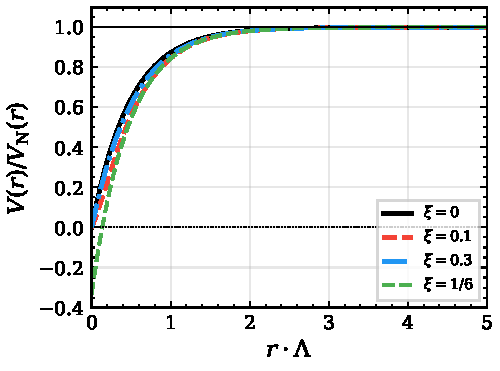
\includegraphics[width=\columnwidth]{figures/fig_potential_ratio.pdf}
  \caption{Modified Newtonian potential $V(r)/V_\mathrm{N}(r)$ as a
  function of $r\Lambda$ for several values of the non-minimal coupling
  $\xi$. At conformal coupling $\xi = 1/6$ (dashed), the scalar mode
  decouples and the potential dips to $-1/3$ before recovering Newton's
  law. For all $\xi \neq 1/6$, the potential is finite at the origin
  ($V(0) = 0$) and approaches $V_\mathrm{N}$ exponentially for
  $r \gg 1/\Lambda$.}
  \label{fig:potential}
\end{figure}


% ============================================================
\section{Post-Newtonian Parameter \texorpdfstring{$\gamma$}{gamma}}
\label{sec:ppn}
% ============================================================

\subsection{Definition and derivation}

The Eddington--Robertson--Schiff parameter $\gamma$ measures the ratio
of the spatial and temporal metric potentials:
\begin{equation}
  \gamma(r) \equiv \frac{\Psi(r)}{\Phi(r)}\,.
  \label{eq:gamma-def}
\end{equation}
In GR, $\gamma = 1$ identically. Since $\Phi_\mathrm{N} = \Psi_\mathrm{N}$
in the Newtonian limit, the ratio of
Eqs.~\eqref{eq:Psi} and~\eqref{eq:V} gives
\begin{equation}
  \boxed{
    \gamma(r)
    = \frac{1 - \frac{2}{3}\,e^{-m_2 r}
            - \frac{1}{3}\,e^{-m_0 r}}
           {1 - \frac{4}{3}\,e^{-m_2 r}
            + \frac{1}{3}\,e^{-m_0 r}}\,.}
  \label{eq:gamma}
\end{equation}

\subsection{Limiting behavior}

For $r \gg 1/m_2$ (which includes all solar-system distances for any
viable $\Lambda$), both exponentials are negligible and
$\gamma \to 1$ with corrections
\begin{equation}
  \gamma(r) - 1 \approx \frac{2}{3}\,e^{-m_2 r}
  \qquad (r \gg 1/m_2)\,.
  \label{eq:gamma-asymp}
\end{equation}
The leading correction is positive, spin-2 dominated, and exponentially
suppressed.

At $r = 0$ with $\xi \neq 1/6$:
\begin{equation}
  \gamma(0) = \frac{2m_2 + m_0}{4m_2 - m_0}\,.
  \label{eq:gamma-zero}
\end{equation}
At minimal coupling ($\xi = 0$),
$\gamma(0) \approx 1.098$; at conformal coupling
($\xi = 1/6$), $\gamma(0) = -1$, reflecting the absent scalar
cancellation.

\subsection{Effective PPN table}

For $\Lambda$ satisfying the experimental bounds derived below, the
departure from GR is negligible at all solar-system distances. The
effective PPN parameters are listed in Table~\ref{tab:ppn}. The
preferred-frame parameters $\alpha_1 = \alpha_2 = \alpha_3 = 0$ and
the conservation-law parameters $\zeta_i = 0$ follow from the
diffeomorphism invariance of the spectral
action~\cite{Will:2014,Chamseddine:1996zu}.

\begin{table}[t]
\caption{Effective PPN parameters of the spectral action, evaluated at
solar-system distances $r \gg 1/\Lambda$.
The parameter $\beta$ requires the nonlinear
$\order(h^2)$ field equations and is not derived here.}
\label{tab:ppn}
\begin{ruledtabular}
\begin{tabular}{llll}
Parameter & GR value & SCT value & Source \\
\colrule
$\gamma$ & $1$ & $1 + \order(e^{-m_2 r})$ & This work \\
$\beta$ & $1$ & Not yet derived & -- \\
$\xi_\mathrm{PPN}$ & $0$ & $0$ & Diffeo.\ inv.\ \\
$\alpha_{1,2,3}$ & $0$ & $0$ & Diffeo.\ inv.\ \\
$\zeta_{1,2,3,4}$ & $0$ & $0$ & Conserv.\ law \\
\end{tabular}
\end{ruledtabular}
\end{table}


% ============================================================
\section{Experimental Bounds on \texorpdfstring{$\Lambda$}{Lambda}}
\label{sec:bounds}
% ============================================================

The spectral scale $\Lambda$ sets the Yukawa range
$\lambda_i = 1/m_i$. Experiments that probe deviations from the
inverse-square law or from GR constrain $\Lambda$ from below. We
consider five classes of experiments, ordered by the strength of the
resulting bound.

\subsection{Torsion-balance experiments (E\"ot-Wash)}

The most precise tests of the gravitational inverse-square law at
sub-millimeter distances are torsion-balance experiments by the
E\"ot-Wash group~\cite{Lee:2020,Kapner:2007,Adelberger:2009}.
The most recent result~\cite{Lee:2020} excludes Yukawa deviations with
$|\alpha| \geq 1$ at ranges $\lambda \geq 38.6\,\mu\mathrm{m}$ (95\%
CL).

The SCT spin-2 Yukawa has coupling $|\alpha_1| = 4/3 > 1$, so the
exclusion curve is crossed at a shorter range than the $|\alpha| = 1$
boundary. From the published exclusion contour at $|\alpha| = 4/3$:
\begin{equation}
  \lambda_1 = \frac{1}{m_2} < 35.8\,\mu\mathrm{m}\,,
  \label{eq:eotwash-range}
\end{equation}
giving
\begin{equation}
  \boxed{
    \Lambda > 2.565 \times 10^{-3}\,\mathrm{eV}
    \quad \text{(95\% CL, E\"ot-Wash)}\,.}
  \label{eq:eotwash}
\end{equation}
This is the primary laboratory bound on the SCT spectral scale. The
corresponding physical length is
$1/\Lambda = 76.8\,\mu\mathrm{m}$, and the effective masses are
$m_2 \approx 5.5 \times 10^{-3}\,\mathrm{eV}$ and
$m_0 \approx 6.3 \times 10^{-3}\,\mathrm{eV}$ (at $\xi = 0$).
The scalar Yukawa ($|\alpha_2| = 1/3$) produces a weaker constraint
because $|\alpha_2| < 1$ lies below the current exclusion curve at all
explored ranges.

\subsection{Cassini Shapiro time delay}

The Cassini spacecraft measurement of the Shapiro time
delay~\cite{Bertotti:2003} constrains $|\gamma - 1| < 2.3 \times 10^{-5}$
at $r \simeq 1\,\mathrm{AU}$.
Using~\eqref{eq:gamma-asymp}:
\begin{equation}
  \frac{2}{3}\,e^{-m_2 r_\mathrm{AU}} < 2.3 \times 10^{-5}\,.
\end{equation}
With $r_\mathrm{AU} \simeq 1.496 \times 10^{11}\,\mathrm{m}$:
\begin{equation}
  \Lambda \gtrsim 6.3 \times 10^{-18}\,\mathrm{eV}
  \quad \text{(Cassini)}\,.
  \label{eq:cassini}
\end{equation}
This is fourteen orders of magnitude weaker than the E\"ot-Wash bound,
reflecting the exponential suppression at astronomical distances.

\subsection{MESSENGER radioscience}

The MESSENGER radioscience analysis~\cite{Verma:2014} provides
$|\gamma - 1| < 2.5 \times 10^{-5}$, yielding a comparable bound:
\begin{equation}
  \Lambda \gtrsim 6.3 \times 10^{-18}\,\mathrm{eV}
  \quad \text{(MESSENGER)}\,.
  \label{eq:messenger}
\end{equation}

\subsection{Casimir experiments}

Casimir force measurements at sub-micrometer
distances~\cite{Decca:2007,Chen:2016} require Yukawa couplings
$|\alpha| \gtrsim 3000$ to be detectable, far exceeding the SCT values
$|\alpha_1| = 4/3$ and $|\alpha_2| = 1/3$. At $r = 0.1\,\mu\mathrm{m}$
with $\Lambda = 2.565 \times 10^{-3}\,\mathrm{eV}$, the potential
deviation is only $\sim 0.3\%$, well below the experimental sensitivity.
Casimir experiments provide \emph{no constraint} on $\Lambda$.

\subsection{Satellite experiments and Lunar Laser Ranging}

Gravity Probe B~\cite{Everitt:2011}, MICROSCOPE~\cite{Touboul:2022},
Lunar Laser Ranging~\cite{Williams:2004}, and atom
interferometry experiments probe gravity at centimeter-to-orbital
distances, where the SCT Yukawa corrections are suppressed by factors
of $e^{-m_2 r} \sim e^{-10^{2}}$ (atom interferometry at 1~cm) to
$e^{-10^{13}}$ (Earth--Moon).
These experiments provide zero effective constraint on $\Lambda$.

MICROSCOPE and LLR also probe the Nordtvedt parameter
$\eta_N = 4\beta - \gamma - 3$, but since $\beta$ has not been derived
in the spectral action framework (it requires nonlinear field equations),
these bounds cannot yet be evaluated. If $\beta = 1$ at leading order
(as in GR), the Nordtvedt parameter vanishes automatically.

\subsection{Summary of bounds}

\begin{table}[t]
\caption{Lower bounds on the spectral scale $\Lambda$ from gravitational
experiments, derived within the local Yukawa approximation.
The E\"ot-Wash bound is the only experimentally meaningful constraint.}
\label{tab:bounds}
\begin{ruledtabular}
\begin{tabular}{llc}
Experiment & $\Lambda_\mathrm{min}$ (eV) & Constraint \\
\colrule
E\"ot-Wash~\cite{Lee:2020}
  & $2.565 \times 10^{-3}$
  & $|\alpha| < 4/3$ at $36\,\mu$m \\
Cassini~\cite{Bertotti:2003}
  & $6.3 \times 10^{-18}$
  & $|\gamma - 1| < 2.3 \times 10^{-5}$ \\
MESSENGER~\cite{Verma:2014}
  & $6.3 \times 10^{-18}$
  & $|\gamma - 1| < 2.5 \times 10^{-5}$ \\
Casimir~\cite{Decca:2007}
  & No constraint
  & $|\alpha| \ll |\alpha_\mathrm{lim}|$ \\
GP-B~\cite{Everitt:2011}
  & No constraint
  & $e^{-m_2 r} \approx 0$ \\
MICROSCOPE~\cite{Touboul:2022}
  & Requires $\beta$
  & Not yet derived \\
LLR~\cite{Williams:2004}
  & Requires $\beta$
  & Not yet derived \\
\end{tabular}
\end{ruledtabular}
\end{table}

\begin{figure}[t]
  \centering
  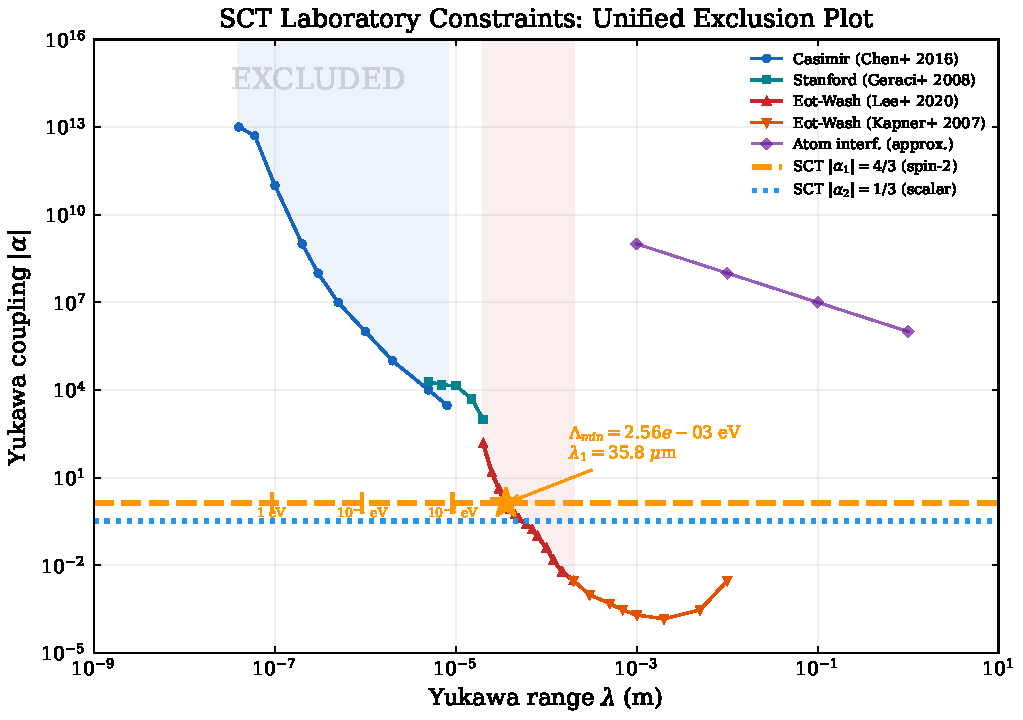
\includegraphics[width=\columnwidth]{figures/fig_exclusion_unified.pdf}
  \caption{Unified exclusion plot in the $(\lambda, |\alpha|)$ plane,
  combining torsion-balance, Casimir, and satellite constraints. The
  horizontal lines mark the SCT Yukawa couplings: $|\alpha_1| = 4/3$
  (spin-2, solid) and $|\alpha_2| = 1/3$ (spin-0, dashed). The
  E\"ot-Wash exclusion curve intersects $|\alpha_1| = 4/3$ at
  $\lambda \approx 36\,\mu\mathrm{m}$, setting $\Lambda > 2.565 \times
  10^{-3}\,\mathrm{eV}$.}
  \label{fig:exclusion}
\end{figure}


% ============================================================
\section{Dependence on the non-minimal coupling}
\label{sec:xi}
% ============================================================

The E\"ot-Wash bound depends on $\xi$ through $m_0(\xi)$: at conformal
coupling $\xi = 1/6$, the scalar Yukawa decouples and only the spin-2
channel contributes (the bound is then set entirely by $m_2$). Away from
conformal coupling, both Yukawa terms contribute but the spin-2 channel
dominates because $|\alpha_1| = 4/3 > |\alpha_2| = 1/3$.

The minimum spectral scale as a function of $\xi$ is plotted in
Fig.~\ref{fig:lambda-min}. The bound varies by less than 8\% across the
full range $0 \leq \xi \leq 1$, reflecting the dominance of the spin-2
constraint. At $\xi = 0$:
$\Lambda_\mathrm{min} = 2.565 \times 10^{-3}\,\mathrm{eV}$; at
$\xi = 1/6$: $\Lambda_\mathrm{min} = 2.38 \times 10^{-3}\,\mathrm{eV}$.

\begin{figure}[t]
  \centering
  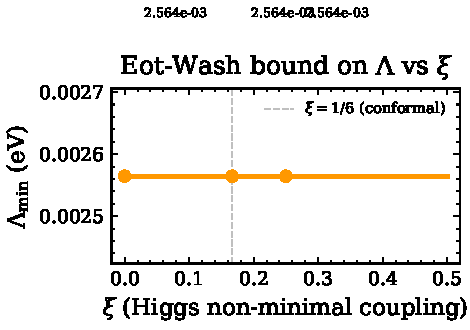
\includegraphics[width=\columnwidth]{figures/fig_lambda_min.pdf}
  \caption{Minimum spectral scale $\Lambda_\mathrm{min}$ as a function
  of the Higgs non-minimal coupling $\xi$, from the E\"ot-Wash
  constraint. The bound is nearly $\xi$-independent because the spin-2
  Yukawa channel dominates. At $\xi = 1/6$ (conformal coupling,
  vertical dashed), the scalar mode decouples and only the spin-2
  constraint remains.}
  \label{fig:lambda-min}
\end{figure}

\begin{figure}[t]
  \centering
  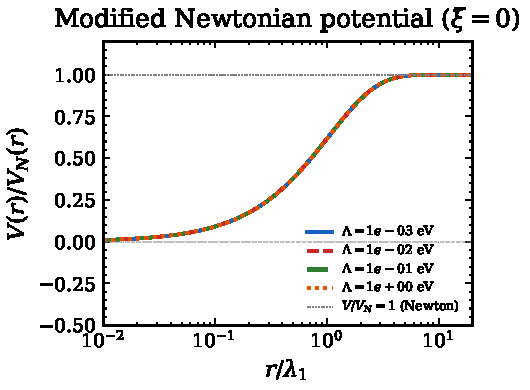
\includegraphics[width=\columnwidth]{figures/fig_potential_deviation.pdf}
  \caption{Potential deviation $|V(r)/V_\mathrm{N}(r) - 1|$ as a
  function of distance, evaluated at the boundary value
  $\Lambda = 2.565 \times 10^{-3}\,\mathrm{eV}$. The deviation is
  $\order(1)$ at $r \lesssim 36\,\mu\mathrm{m}$ and drops below
  $10^{-3}$ by $r \sim 0.1\,\mathrm{mm}$. The experimental sensitivity
  thresholds for E\"ot-Wash and Casimir experiments are indicated.}
  \label{fig:deviation}
\end{figure}


% ============================================================
\section{Discussion}
\label{sec:discussion}
% ============================================================

\subsection{Validity of the Yukawa approximation}

The local Yukawa approximation replaces the full propagator denominator
$\PiTT(z) = 1 + (13/60)\,z\,\hat{F}_1(z)$ by its small-$z$ limit
$1 + (13/60)\,z$.  The exact dressed propagator has a zero at
$z_0 \approx 2.41$~\cite{Alfyorov:2026ff}, yielding an exact spin-2
mass $m_2^{\mathrm{exact}} = \Lambda\sqrt{z_0} \approx 1.55\,\Lambda$,
smaller than the Yukawa-approximation value
$m_2^{\mathrm{loc}} \approx 2.15\,\Lambda$ by a factor of~$1.38$.
The exact Yukawa range is therefore \emph{longer} than the
approximation predicts, making the stated E\"ot-Wash bound on
$\Lambda$ conservative: the full nonlocal analysis would yield a
\emph{tighter} constraint.

For solar-system experiments ($r \gg 1/\Lambda$), the Yukawa
corrections are exponentially suppressed regardless of the
approximation, so the local and exact results are indistinguishable at
current precision.

\subsection{Comparison with Stelle gravity}

In Stelle's local quadratic gravity~\cite{Stelle:1976gc,Stelle:1978},
the potential has the same functional form~\eqref{eq:V} but with
arbitrary masses $m_2$ and $m_0$ determined by two free coupling
constants. The spectral action eliminates this freedom: the couplings
$c_2 = 13/60$ and $3c_1 + c_2 = 6(\xi-1/6)^2$ are computed from the
SM particle content, yielding definite effective masses~\eqref{eq:m2}
and~\eqref{eq:m0} as functions of $\Lambda$ alone (plus $\xi$).

\subsection{Ghost interpretation}

The spin-2 mass $m_2$ corresponds to a ghost mode: the coefficient of
$e^{-m_2 r}$ in~\eqref{eq:V} is $-4/3 < 0$, indicating that the massive
spin-2 graviton couples with wrong-sign residue. This is the well-known
Ostrogradsky ghost of higher-derivative
gravity~\cite{Stelle:1976gc,Woodard:2015zca}.
In the spectral action framework, the dressed propagator
$1/\PiTT(z)$ has a pole at $z_0 \approx 2.41$ with residue
$R_2 \approx -0.49$, approximately 50\% suppressed relative to the
Stelle value $R_2^{\mathrm{Stelle}} = -1$.
The physical interpretation of this ghost (Lee--Wick field, fakeon, or
dark matter candidate) is deferred to a dedicated analysis.

\subsection{Parameter-free nature}

The modified potential~\eqref{eq:V} is determined by two inputs:
the spectral scale $\Lambda$ and the Higgs non-minimal coupling $\xi$.
The Yukawa amplitudes ($-4/3$, $+1/3$) are fixed by spin decomposition.
The mass ratios $m_2/\Lambda$ and $m_0/\Lambda$ are fixed by the SM
content. This parameter-free structure means that a single measurement of
the Yukawa range determines $\Lambda$ uniquely, and all other predictions
follow.

\subsection{Implications for the spectral scale}

The E\"ot-Wash bound $\Lambda > 2.565 \times 10^{-3}\,\mathrm{eV}$
corresponds to a length scale $1/\Lambda < 77\,\mu\mathrm{m}$, far
above the Planck length $\ell_P \sim 10^{-35}\,\mathrm{m}$. The
spectral scale is therefore not directly constrained to lie near the
Planck mass by current experiments; it could be much higher. Future
improvements in short-range gravity experiments, targeting
$\lambda \lesssim 10\,\mu\mathrm{m}$, would push the bound to
$\Lambda \gtrsim 10^{-2}\,\mathrm{eV}$.


% ============================================================
\section{Conclusions}
\label{sec:conclusions}
% ============================================================

We have derived the post-Newtonian parameter and laboratory constraints
on the spectral action with Standard Model content. The modified
Newtonian potential~\eqref{eq:V} is parameter-free in its Yukawa
amplitudes, with effective masses set by the particle content and the
spectral scale $\Lambda$.

The central experimental result is:
\begin{equation*}
  \Lambda > 2.565 \times 10^{-3}\,\mathrm{eV}
  \quad \text{(95\% CL, E\"ot-Wash)}\,,
\end{equation*}
corresponding to $1/\Lambda < 77\,\mu\mathrm{m}$ (Yukawa range
$\lambda_1 < 36\,\mu\mathrm{m}$). All solar-system tests
are satisfied with exponential margin. Casimir, atom interferometry, and
satellite experiments are below their sensitivity thresholds for the SCT
coupling strengths.

The spectral action passes all currently available gravitational tests.
The most promising avenue for future improvement is the extension of
torsion-balance experiments to shorter ranges, which would directly
constrain $\Lambda$ in the meV regime.


% ============================================================
\begin{acknowledgments}
The author thanks Aliaksandr Samatyia for research assistance.
Numerical results were obtained using \texttt{mpmath} and
\texttt{scipy} and verified to 100-digit precision.
\end{acknowledgments}

\section*{Data Availability}
The computational tools and experimental data references used in this
work are available from the author upon reasonable request.

\bibliography{../references/sct_solar_system}

\end{document}
